%% LyX 2.1.1 created this file.  For more info, see http://www.lyx.org/.
%% Do not edit unless you really know what you are doing.
\documentclass[12pt,english]{article}
\usepackage[T1]{fontenc}
\usepackage[latin9]{inputenc}
\usepackage[a4paper]{geometry}
\geometry{verbose,tmargin=1.25cm,bmargin=1.25cm,lmargin=1.25cm,rmargin=1.25cm,headheight=1.25cm,headsep=1.25cm,footskip=1.25cm}
\usepackage{graphicx}
\usepackage{babel}
\begin{document}

\title{Week 1:FDM Applied to Solve Laplace Equation\\
for Systems with Finite Boundary Conditions}


\author{Sankeerth.D\\
EE13B102\\
Electrical Engineering}
\maketitle
\begin{abstract}
Finite Difference Method (FDM), used to numerically solve differential
equations by approximating derivatives as differences. Here, it is
used to solve an 2D electrostatic problem where one edge of a rectangle
is given a nonzero voltage and the other three edges are grounded.
The simulation has been performed in MATLAB, where two approaches
have been used to calculate the iterations. Analysis of the simulation
have also been done.
\end{abstract}

\section{Introduction}

FDM approximates the second derivative at a point as the average of
the four surrounding points:
\begin{description}
\item [{
\[
\nabla^{2}V=0
\]
}]~
\item [{
\[
V_{i,j}=\frac{V_{i,j-1}+V_{i,j+1}+V_{i-1,j}+V_{i+1,j}}{4}
\]
}]~
\end{description}
At the boundary, the V value is not updated. The given area is split
into a rectangular grid of points, and the derivative can be computed
at these points using the above approximation. These above conditions
can be put into an algorithm.


\section{Implimentation}

One possible algorithm which converges would be to initialize all
voltages to zero in the beginnning, and then starting from the first
point, using the above average , compute the updated value. then move
to the adjascent point and compute the average again and so on. Carry
our this process after sufficient number of iterations. This way of
implementation is done in the program with for loop, where the for
loops are used to iterate through the grid points.

Another way is to caculate average of each point with the surrounding
points' in the grid, and then update the values all at once. Then
continue with the iteration. This has been implimented using the matrix
operations available in MATLAB, and the implementation turns out to
be elegant.

One would expect the first method would use fewer number of iterations
than the second as we're updating the values at a slower rate. But
since 'for' loops in MATLAB are costly when in comes to computation
time, the second method might take lesser time than the first.


\section{Observation}

Both the algorithms converge and yield reasonable solutions. The iterations
have been carried out for the number of points ranging from 20X20
to 100X100, at steps of 5. The numerical solution obtained is as follows
(for a 100X100 grid):

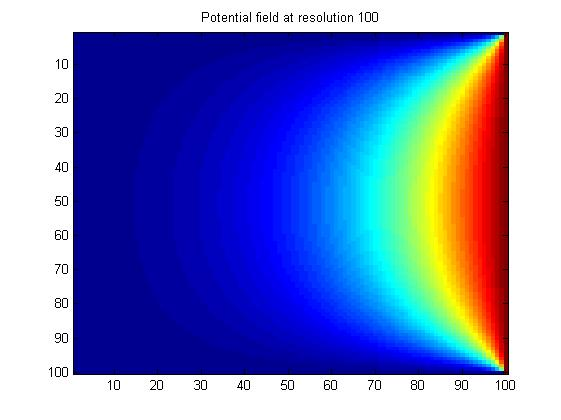
\includegraphics{potential}

The normallized Electric Field with its direcrtion is as shown(taken
from solution for 30X30 grid):

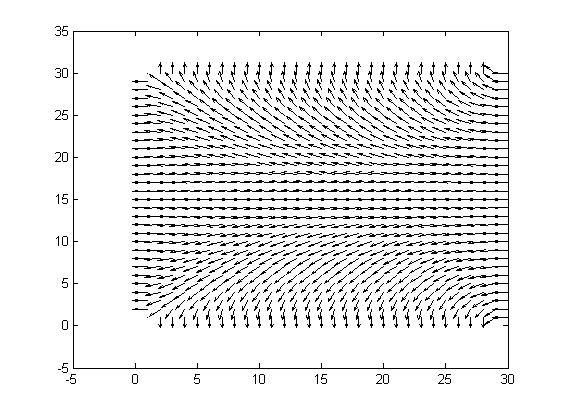
\includegraphics{field} 

As one can notice, the boundary conditions are satisfied as the electric
field is perpendicular to the edges.


\section{Analysis of algorithms}

When using the for loop algorithm, the following time and number of
iterations characteristics are obtained with respect to grid size(on
one axis):

\includegraphics{\string"time using for loop\string".jpg} \includegraphics{\string"iterations using for loop\string".jpg}

As one can see, it takes around 2 seconds to run through around 1500
iterations for a 100X100 grid.

For the second algorithm, the corresponding time and number of iterations
characteristics versus the grid size is as follows:

\includegraphics{\string"time no loop\string".jpg} \includegraphics{\string"iterations no loop\string".jpg}

Even the 100X100 grid takes 0.35 millisecconds on the second algorithm,
which ran 1850 iterations.


\section{Result and Discussion}

From the graphs, using the for loop algorithm, the time taken varies
almost parabolically with the grid size, that is, it grows linerly
with the number of grid points. This seems reasonable as each time
it iterates through each point inside the for loop. Also, since the
for loop is inefficient in MATLAB, it's effect can be observed as
it takes a full 2 seconds to compute solution for the 100X100 grid.

As with the other case, as expecte, it has many number of iterations
than the first one, but it has much lesser execution time, around
0.3 seconds even for the 100X100 case, since it was done sing the
matrix operations offered my MATLAB. Also, it an be seen, the execution
time is closer to a linear graph in this case, unlike the squared
case in the one above. 
\end{document}
